\documentclass[11pt,titlepage,fleqn]{article}

\usepackage{amsmath}
\usepackage{amssymb}
\usepackage{latexsym}
\usepackage[round]{natbib}
\usepackage{xspace}
\usepackage{graphicx}
%\usepackage{epsfig}

\usepackage{pifont}   % search for \ding

%\usepackage{fancyhdr}
%\pagestyle{fancy}

%=====================================================
%       SPACING COMMANDS (Latex Companion, p. 52)
%=====================================================

\usepackage{setspace}

%---------------------------
\newcommand{\matlab}{\textsc{Matlab}\xspace}
%---------------------------
\renewcommand{\baselinestretch}{1.0}

\textwidth 460pt
\textheight 700pt
\oddsidemargin 0pt
\evensidemargin 0pt

% see Latex Companion, p. 85
\voffset     -50pt
\topmargin     0pt
\headsep      20pt
\headheight    0pt
\footskip     30pt
\hoffset       0pt

\include{carlcommands}
%\input{dp_header}

\graphicspath{
  {/home/vipul/REPOSITORIES/IITR_seismo/classes/ES510/latex/figures/}
  }

\begin{document}

\noindent Course: Numerical Methods and Computer Programming\\
\noindent Code: ES 510\\
\noindent Instructor: Vipul Silwal (\verb+vsilwalfes@iitr.ac.in+) \\ 
\noindent Last Compiled: \today \\

{\huge Numerical integration and differentiation}

\tableofcontents 
%% ------------------------------------------------------------------------ %%


\begin{section}{Numerical Derivative}
{\bf Newton forward}
\begin{equation}
f'(x) \simeq \frac{f(x+h) - f(x)}{h}
\end{equation}
{\bf Stirling}
\begin{equation}
f'(x) \simeq \frac{f(x+h) - f(x-h)}{2h}
\end{equation}
{\bf Newton backward}
\begin{equation}
f'(x) \simeq \frac{f(x) - f(x-h)}{h}
\end{equation}

\underline{\bf Double Derivate}
Using Newton forward and Newton backward:
\begin{eqnarray}
f''(x) &=& \frac{\frac{f(x+h) - f(x)}{h} - \frac{f(x) - f(x-h)}{h}}{h}\\
&=& \frac{f(x+h) - 2f(x) + f(x-h)}{h^2}
\end{eqnarray}
\end{section}
%-----------------------------------------------------

\begin{section}{Numerical Integration and Quadrature Rules}
A quadrature rule is an approximation of the definite integral of a function, usually stated as weighted sum of function values at specified points within the domain of integration (source: wiki).

\begin{subsection}{Midpoint rule}
Also known as {\bf Riemann sum}. In this we divide the entire summation range $[a,b]$ into $N$ number of small rectanges.$[x_0,x_1], [x_0,x_1], \cdots [x_{N-1},x_N]$; with discretiation interval $h = \frac{x_N - x_0}{N} = (x_1 - x_0)$.

The area in this case could be approximated as:

\begin{equation}
A = h * f(\frac{x_0 + x_1}{2}) + h * f(\frac{x_1 + x_2}{2}) + \cdots + h * f(\frac{x_{N-1} + x_N}{2})
\end{equation}

As the discretization $h$ decreases, the summation results get closer to what is called {\it Reimann integral}.

\end{subsection}

%---------------------------------------------------------
\begin{subsection}{Trapezoidal Rule}
In this we approximate the area under the curve using numerous trapezoids.

For example, the area under the parabola in the following figure could be approximated using only two trapezoids (3 points):
\begin{eqnarray}
A &=& \frac{1}{2} h (y_0 + y_1) + \frac{1}{2} h (y_1 + y_2)\\
A &=& \frac{1}{2} h (y_0 + 2 y_1 + y_2)
\end{eqnarray}
where $h$ is the space between the points on x-axis; and $y_0 = f(x_0), y_1
 = f(x_1), y_2 = f(x_2)$.

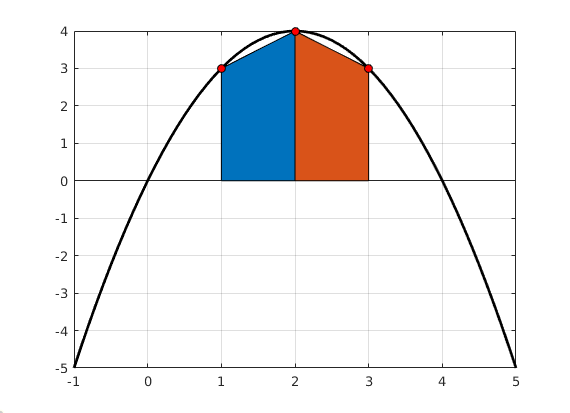
\includegraphics[scale=0.75]{trapezoid.png} \label{trap}

Similary using 5 points (4 trapezoids) the area would be:
\begin{eqnarray}
A &=& \frac{1}{2} h (y_0 + y_1) + \frac{1}{2} h (y_1 + y_2) + 
\frac{1}{2} h (y_2 + y_3) + \frac{1}{2} h (y_3 + y_4) \\
A &=& \frac{1}{2} h (y_0 + 2 y_1 + 2y_2 + 2y_3 + y_4)
\end{eqnarray}

\underline{General Form:} 
\begin{equation}
A = \frac{1}{2} h (y_0 + 2 y_1 + 2y_3 + \cdots + 2y_{N-1} + y_N)
\end{equation}
\end{subsection}

\begin{subsection}{Simpson's Rule}
Also known as {\bf Newton-Cotes quadrature rule} or {\bf Kepler's rule}. Unlike the previous two methods where we approximated the curve using rectangular blocks and trapezoids, here we use {\it quadratic functions} instead. Of the three, this gives the most accurate results.

\underline{Derivation:} (\verb+obtained from Igor Yanovsky's webapge, UCLA+)
\begin{eqnarray*}
\int_{x_0}^{x_2} f(x) dx &=& \int_{x_0}^{x_2} [ f(x_1) + f'(x_1)(x - x_1) + \frac{f''(x_1)}{2!}(x - x_1)^2 \\
&&+ \frac{f'''(x_1)}{3!}(x - x_1)^3 + \frac{f''''(\xi)}{4!}(x - x_1)^4  ] dx \\
&=&  [ f(x_1)x + \frac{f'(x_1)}{2}(x - x_1)^2 + \frac{f''(x_1)}{3 \cdot 2!}(x - x_1)^3 \\
&& + \frac{f'''(x_1)}{4 \cdot .3!}(x - x_1)^4 + \frac{f''''(\xi)}{5\cdot4!}(x - x_1)^5  ]_{x_0}^{x_2}  \\
&=&  [ f(x_1)(x_2 - x_0) + \frac{f'(x_1)}{2}[(x_2 - x_1)^2 - (x_0 - x_1)^2] \\
&& + \frac{f''(x_1)}{6}[(x_2 - x_1)^3 - (x_0 - x_1)^3] + \frac{f'''(x_1)}{24}[(x_2 - x_1)^4 - (x_0 - x_1)^4] \\
&& + \frac{f''''(\xi)}{120}[(x_2 - x_1)^5 - (x_0 - x_1)^5] \\
&=& 2h f(x_1) + \frac{f'(x_1)}{2}[h^2 - h^2] + \frac{f''(x_1)}{6}[h^3 + h^3] \\
&& + \frac{f''(x_1)}{24}[h^4 - h^4] + \frac{f''''(\xi)}{120}[h^5 + h^5] \\
&=& 2h f(x_1) + h^3 \frac{f''(x_1)}{3} + h^5\frac{f''''(\xi)}{60} \\
&=& 2h f(x_1) + \frac{h^3}{3} \left [ \frac{f(x_0) - 2f(x_1) + f(x_2)}{h^2} \right ] + E \\
&=& \frac{h}{3} \left [ f(x_0) + 4f(x_1) + f(x_2)\right]
\end{eqnarray*}

\end{subsection}
\end{section}
%-----------------------------------------------------

\begin{section}{Discretizing Integral equation (and Geophysical Application)}
The first step towards performing numerical integration is discretizing the analytical equation into its numerical form.

Consider the following equation:
\begin{equation}
d(x) = \int_a^b g(x,\xi)m(\xi)d\xi
\end{equation}
This is called a Fredholm integral equation of the first kind (or IFK), which is frequenctly used in Geophysics to describe a model. $d(x)$ is a function that represent the data (however, the observed data will only be present at few selected points); $g(x,\xi)$ represents a mathematical relation that maps model paramters $m(\xi)$ onto the data space. $\xi$ is element representative of model parameter space.

This could also be written as:
\begin{equation}
d_i = d(x_i) = \int_a^b g_i(x) m(x) dx
\end{equation}

Now divide the interval $[a,b]$ into $n$ intervals. 
\begin{equation}
\Delta x = \frac{b-a}{n}
\end{equation}

By applying {\bf mid-point rule} for finding the area, 
\begin{equation}
d_i = \int_a^b g_i(x) m(x) dx \approx \sum_{j=1}^n g_i(x_j)m(x_j)\Delta x
\end{equation}
where we only need to know value of $g(x_j)$ and $m(x_j)$ at $n$ points.

This could further be condensed to:
\begin{eqnarray}
d_i &=& \sum_{j=1}^n G_{i,j} m_j \\
\bd &=& \bG \bem
\end{eqnarray}

\end{section}

%-----------------------------------------------------
\begin{section}{Exercise}
\begin{enumerate}
\item 
\begin{itemize}
\item Using the same example provided in Figure \ref{trap} extend the {\bf trapezoidal rule} to 5 points. Hint: Use the lab's \matlab example to get started.
\item Using \matlab function \verb+trapz+ compute the area (more accurate approximation) and compare the difference.
\end{itemize}

\item Compute the integrals of following functions and then compare with Simpson's rule :
\begin{itemize}
\item $f(x) = 2x^3 - 4x^2 + 3x -1, x \in [-1, 3]$
\item $f(x) = \sin x, x \in [0,\frac{\pi}{3}]$
\end{itemize}

\item In vertical seismic profiling, we wish to know the velocity of material sourrounding the borehole. A downward-propagating wavefront is generated at the surface by a source, and seismic waves are sensed by a string of seismometers in the borehole.

The arrival times of the seismic wavefront at each instrument, which reflects the seismic velocity for vertically travelling waves as a function of depth are measured from the recorded seismograms.
\begin{eqnarray}
t(z) &=& \int_0^z s(\xi) d\xi \\
&=& \int_0^\infty s(\xi) H(z - \xi) d\xi
\end{eqnarray}
where $H$ is the heaviside function, and s(z) is the slowness (reciprocal of the velocity). The slowness was used instead of velocity to linearize the equation (application of change of parameterization).

\underline{Problem: } Discretize this equation, considering there are $N$ number of seismometer, and hence you will have $N$ arrival times. (If you performed inverion, you would have been able to get velocity at $N$ depths).

\end{enumerate}
\end{section}
%-----------------------------------------------------
\end{document}
